\section{Heterogeneous Treatment Effects}

\begin{frame}{A Set of Spatial Treatment Effects}
\begin{itemize}
    \item Assume we have finite spatial grid which is divided in $i∗j$ grids, where $i \in Lat$ and $j \in Long$. 
    \vspace{-7pt}
    \item Then, we can obtain a set of treatment effects $D = \{\delta_{1,1}, \delta_{2,1}, \delta_{1,2}, ..., \delta_{i,j}\}$ by subtracting synthetic untreated outcomes in observed treated outcomes at position $i,j$. 
    \vspace{-7pt}
    \item Commonly, it is assumed that all elements of $D$ are constant over space. This assumption does not hold in spatially heterogeneous settings.
\end{itemize}
\end{frame}

\begin{frame}{Reporting Heterogeneous Treatment Effects}

The set of treatment effects $D$ at time $t_i$ may be spatially heterogeneous:  
\vspace{5pt}

  \begin{columns}
    % Split 1
      \begin{column}{0.45\linewidth}
      \centering
      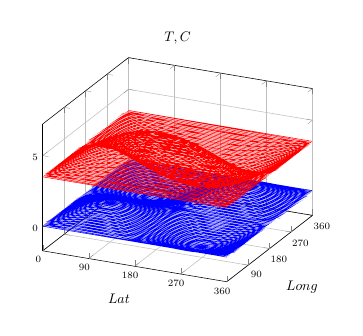
\begin{tikzpicture}[scale=0.50]
      \begin{axis} [
        title = {$T, C$},
        xtick = {0,90,...,360},
        ytick = {90,180,...,360},
        xlabel = $Lat$, ylabel = $Long$,
        ticklabel style = {font = \scriptsize},
	grid]
        \addplot3 [blue, domain=0:360, samples=60] 
        	{ sin(x)*sin(y) };
        \addplot3 [red, domain=0:360, samples=60] 
        	{ sin(0.5*x)*3*sin(y) + 3.5 };
        \end{axis}
        \end{tikzpicture} \\
        \centering{\footnotesize{\textcolor{red}{Treated ($T$)}, \textcolor{blue}{Control ($C$)}}}
    \end{column}
    % Split 2
    \begin{column}{0.45\linewidth}
    \centering
      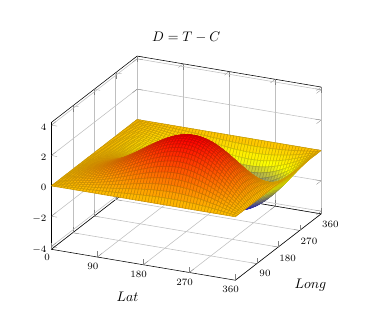
\begin{tikzpicture}[scale=0.50]
      \begin{axis} [
        title = {$D = T - C$},
        xtick = {0,90,...,360},
        ytick = {90,180,...,360},
        xlabel = $Lat$, ylabel = $Long$,
        ticklabel style = {font = \scriptsize},
	grid]
        \addplot3 [surf, domain=0:360, samples=60] 
        	{ sin(0.5*x)*3*sin(y) - sin(x)*sin(y) };
        \end{axis}
        \end{tikzpicture} \\
        \centering{\footnotesize{\textcolor{orange}{Treatment Effects ($D$)}}}
    \end{column}
  \end{columns}
\end{frame}

\begin{frame}{Reporting Heterogeneous Treatment Effects}
\begin{itemize}
    \item How do we report these heterogeneous treatment effects?
    \vspace{-7pt}
\begin{itemize}
    \item Individual Treatment Effect: We report $\delta_{i,j}$ for $\forall i,j$.
    \item Average Treatment Effect: We report $\frac{1}{n}*\sum(\delta_{i,j})$ $\forall i,j$. 
\end{itemize}
    \vspace{-7pt}
    \item The options are unrealistic and uninformative, respectively. Therefore, can we find a good middle ground?
\end{itemize}

\begin{center}
    Formally: We are looking to report the average of k subsets of $D$, where $1 < k < n$ in a plane with $n$ grids. 
\end{center}
\end{frame}

\begin{frame}{The Clustering Problem}
    Rather than pre-define the reporting veracity (e.g., zip code), a clustering approach may allow the data to tell the whole story. 
    \vspace{5pt}

  \begin{columns}
    % Split 1
      \begin{column}{0.6\linewidth}
      \begin{itemize}
          \item How do we find the optimal k?
          \vspace{-7pt}
          \item Problem: As $n$ increases, the error function monotonically decreases
          \vspace{-7pt}
          \item Formally: $\nexists k$ s.t. $argmin_{k}$(Error), outside of $k = n$. 
      \end{itemize}
    \end{column}
    % Split 2
    \begin{column}{0.45\linewidth}
        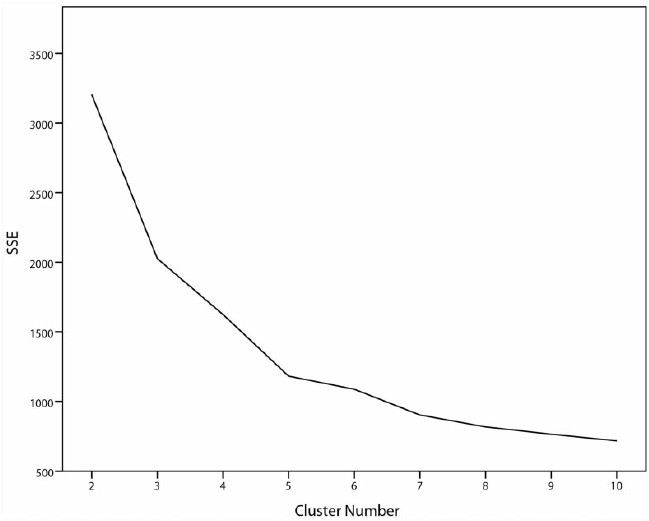
\includegraphics[scale = 0.21]{figures/sse_cluster-n_tradeoff.jpg}\\
        \mycaption{Trade-Off: SSE vs. Cluster #}
    \end{column}
  \end{columns}
\end{frame}

\begin{frame}{A Solution?}
Rather than pre-define the reporting veracity (e.g., zip code), a clustering approach may allow the data to tell the whole story. 
\vspace{5pt}

  \begin{columns}
    % Split 1
      \begin{column}{0.6\linewidth}
      \begin{itemize}
          \item Methods to find $k$: Elbow, Silhouette, etc.
          \vspace{-7pt}
          \item Problem: Curse of dimensionality!
          \vspace{-7pt}
          \item Uncertain: Is time really that important in short time horizons? 
      \end{itemize}
    \end{column}
    % Split 2
    \begin{column}{0.45\linewidth}
        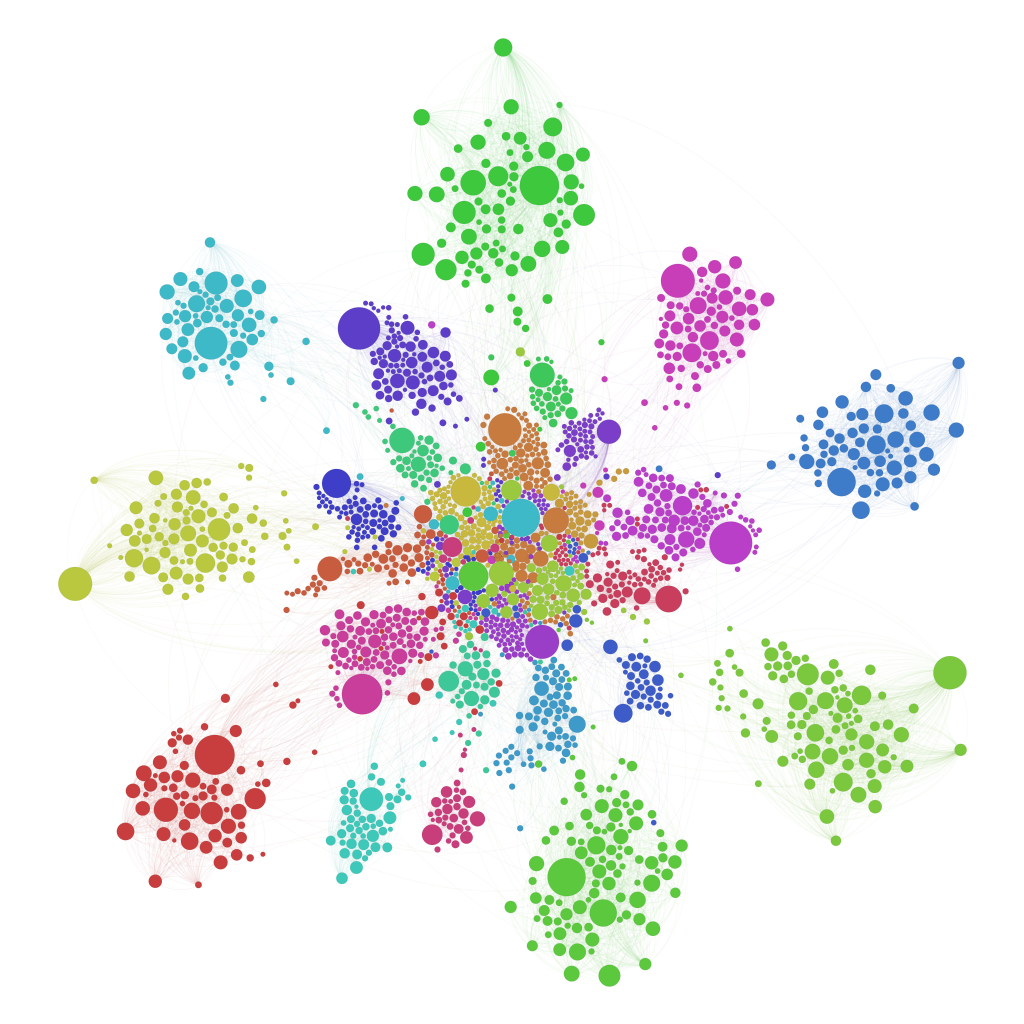
\includegraphics[scale = 0.12]{figures/high-dim_clustering.jpg}\\
        \mycaption{High-dimensional Clustering}
    \end{column}
  \end{columns}
\end{frame}